\section{Casi d'uso}

\subsection{Attori dei casi d'uso}

\subsubsection{Attori primari}
\begin{figure}[H]
		\centering
		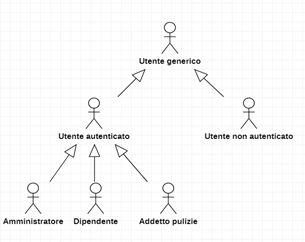
\includegraphics[width=10cm]{res/images/utentigenerali.png}
		\caption{Gerarchia degli attori principali}
		\label{fig:Gerarchia attori principali}
	\end{figure}

\textbf{Utente generico}\\
Si riferisce ad un utente generico che accede alla piattaforma.\\
\\
\textbf{Utente non autenticato}\\
Si riferisce ad un utente generico che non ha ancora effettuato l’autenticazione alla piattaforma.\\
\\
\textbf{Utente autenticato}\\
Si riferisce ad un utente generico che si è autenticato nel sistema con la procedura di login.\\
\\
\textbf{Amministartore}\\
Si riferisce ad un utente che si è autenticato nel sistema con il ruolo di amministratore.\\
\\
\textbf{Dipendente}\\
Si riferisce ad un utente che si è autenticato nel sistema con il ruolo di dipendente.\\
\\
\textbf{Addetto pulizie}\\
Si riferisce ad un utente che si è autenticato nel sistema con il ruolo di addetto alle pulizie.\\

\subsubsection{Attori secondari}
\textbf{Tag RFID}\\
Si riferisce ai tag presenti sulle postazioni. Ogni tag è assegnato ad una postazione e permette di identificarla digitalmente.\\
\\
\textbf{Ethereum}\\
Si riferisce al servizio che memorizza su blockchain gli eventi di occupazione e igienizzazione delle postazioni.\\

\subsection{Elenco dei casi d'uso}
In questa sezione sono riportati tutti i casi d'uso individuati, divisi per attore principale. Quando ritenuto utile essi sono accompagnati da un grafico.
\\
\subsubsection{ UC1 - Guida introduttiva}
\begin{itemize}
           	\item\textbf{Attori Primari:} 
           	\item\textbf{Descrizione:} 
           	\item\textbf{Scenario principale:} 
           	\item\textbf{Precondizione:} 
           	\item\textbf{Postcondizione:}
\end{itemize}

\subsubsection{ UC2 - Login}
\begin{itemize}
           	\item\textbf{Attori Primari:} 
           	\item\textbf{Descrizione:} 
           	\item\textbf{Scenario principale:} 
           	\item\textbf{Precondizione:} 
           	\item\textbf{Postcondizione:}
\end{itemize}

\subsubsection{ UC3 - Logout}
\begin{itemize}
           	\item\textbf{Attori Primari:} 
           	\item\textbf{Descrizione:} 
           	\item\textbf{Scenario principale:} 
           	\item\textbf{Precondizione:} 
           	\item\textbf{Postcondizione:}
\end{itemize}

\subsubsection{ UC4 - Gestione impostazioni}
\begin{itemize}
           	\item\textbf{Attori Primari:} 
           	\item\textbf{Descrizione:} 
           	\item\textbf{Scenario principale:} 
           	\item\textbf{Precondizione:} 
           	\item\textbf{Postcondizione:}
\end{itemize}

\subsubsection{ UC5 - Gestione stanze e postazioni}
\begin{itemize}
           	\item\textbf{Attori Primari:} 
           	\item\textbf{Descrizione:} 
           	\item\textbf{Scenario principale:} 
           	\item\textbf{Precondizione:} 
           	\item\textbf{Postcondizione:}
\end{itemize}
\subsubsection{ UC5.1 - Visualizzazione stanze e postazioni}
\begin{itemize}
	\item\textbf{Attori Primari:}
	Amministratore\\ 
	\item\textbf{Descrizione:}
	Il sistema mostra all'amministratore lo schema delle stanze e delle postazioni aggiornato rispetto alle azioni salvata su Ethereum.
	\item\textbf{Scenario principale:}
	Il sistema ottiene da Ethereum la lista delle azioni salvate. In base a questa aggiorna lo schema delle stanze e delle postazioni e lo fa visualizzare all'amministratore. Le postazioni sono colorate in base al loro stato e gli stati possibili sono:
	- libera e igienizzata
	- libera e non igienizzata
	- occupata
	- prenotata e igienizzata
	- prenotata e non igienizzata
	\item\textbf{Precondizione:} 
	L'utente è autenticato come amministratore.
	\item\textbf{Postcondizione:}
	L'amministratore visualizza lo schema delle stanze e delle postazioni.
\end{itemize}

\subsubsection{ UC6 - Gestione credenziali dipendenti e addetti}
\begin{itemize}
           	\item\textbf{Attori Primari:} 
           	\item\textbf{Descrizione:} 
           	\item\textbf{Scenario principale:} 
           	\item\textbf{Precondizione:} 
           	\item\textbf{Postcondizione:}
\end{itemize}

\subsubsection{ UC7 - Esplorazione postazioni occupate da specifico utente}
\begin{itemize}
           	\item\textbf{Attori Primari:} 
           	\item\textbf{Descrizione:} 
           	\item\textbf{Scenario principale:} 
           	\item\textbf{Precondizione:} 
           	\item\textbf{Postcondizione:}
\end{itemize}

\subsubsection{ UC8 - Report sanificazioni postazione}
\begin{itemize}
           	\item\textbf{Attori Primari:} 
           	\item\textbf{Descrizione:} 
           	\item\textbf{Scenario principale:} 
           	\item\textbf{Precondizione:} 
           	\item\textbf{Postcondizione:}
\end{itemize}

\subsubsection{ UC9 - Visualizza stato postazione}
\begin{itemize}
           	\item\textbf{Attori Primari:} 
           	\item\textbf{Descrizione:} 
           	\item\textbf{Scenario principale:} 
           	\item\textbf{Precondizione:} 
           	\item\textbf{Postcondizione:}
\end{itemize}

\subsubsection{ UC10 - Segnalazione presenza}
\begin{itemize}
           	\item\textbf{Attori Primari:} 
           	\item\textbf{Descrizione:} 
           	\item\textbf{Scenario principale:} 
           	\item\textbf{Precondizione:} 
           	\item\textbf{Postcondizione:}
\end{itemize}

\subsubsection{ UC11 - Pulizia autonoma}
\begin{itemize}
           	\item\textbf{Attori Primari:} 
           	\item\textbf{Descrizione:} 
           	\item\textbf{Scenario principale:} 
           	\item\textbf{Precondizione:} 
           	\item\textbf{Postcondizione:}
\end{itemize}

\subsubsection{ UC12 - Prenotazione postazione}
\begin{itemize}
           	\item\textbf{Attori Primari:} 
           	\item\textbf{Descrizione:} 
           	\item\textbf{Scenario principale:} 
           	\item\textbf{Precondizione:} 
           	\item\textbf{Postcondizione:}
\end{itemize}

\subsubsection{ UC13 - Elenco stanze e postazioni da igienizzare}
\begin{itemize}
           	\item\textbf{Attori Primari:} 
           	\item\textbf{Descrizione:} 
           	\item\textbf{Scenario principale:} 
           	\item\textbf{Precondizione:} 
           	\item\textbf{Postcondizione:}
\end{itemize}

\subsubsection{ UC14 - Marcatura stanza e postazione come igienizzata}
\begin{itemize}
           	\item\textbf{Attori Primari:} 
           	\item\textbf{Descrizione:} 
           	\item\textbf{Scenario principale:} 
           	\item\textbf{Precondizione:} 
           	\item\textbf{Postcondizione:}
\end{itemize}